\documentclass[10pt]{beamer}
\usetheme{jambro}

\title[]{Pensamento Econômico Contemporâneo - A escola Keynesiana ortodoxa}
\author[]{Paulo Victor da Fonseca}
\date{}

\hypersetup{
    colorlinks = true,
    urlcolor = teal,
    linkcolor = teal    
}
\usepackage[portuguese]{babel}
\usepackage{subfig}
\usepackage{emoji}

\begin{document}

\begin{frame}[plain]
    \titlepage{
        \begin{center}
            \begin{minipage}{0.8\textwidth}
                \centering
            \end{minipage}
        \end{center}}
\end{frame}

\begin{frame}{Sumário}
    \tableofcontents
\end{frame}

\section{Modelo IS-LM: economia fechada}
\subsection{Equilíbrio de subemprego no modelo Keynesiano}
\begin{frame}{Equilíbrio de subemprego - IS-LM: caso geral}
    \begin{itemize}
        \item IS-LM: existência de equilíbrio de subemprego pode ser atribuída à existência de algum tipo de `rigidez'
        \bigskip
        \item Especialmente a rigidez de dois preços fundamentais: salário nominal e taxa de juros
        \bigskip
        \item Iniciaremos análise de equilíbrio de subemprego com a hipótese `Keynesiana' de rigidez na redução de salários nominais
        \bigskip
        \item Diagrama de quadro quadrantes:
        \bigskip
        \begin{enumerate}
            \item Modelo IS-LM convencional.
            \medskip
            \item Função de produção agregada de curto prazo.
            \medskip
            \item Mercado de trabalho.
            \medskip
            \item Quadrante auxiliar com linha de 45º.
        \end{enumerate}
    \end{itemize}
\end{frame}

\begin{frame}{Equilíbrio de subemprego - IS-LM: caso geral}
    \begin{figure}
        \centering
        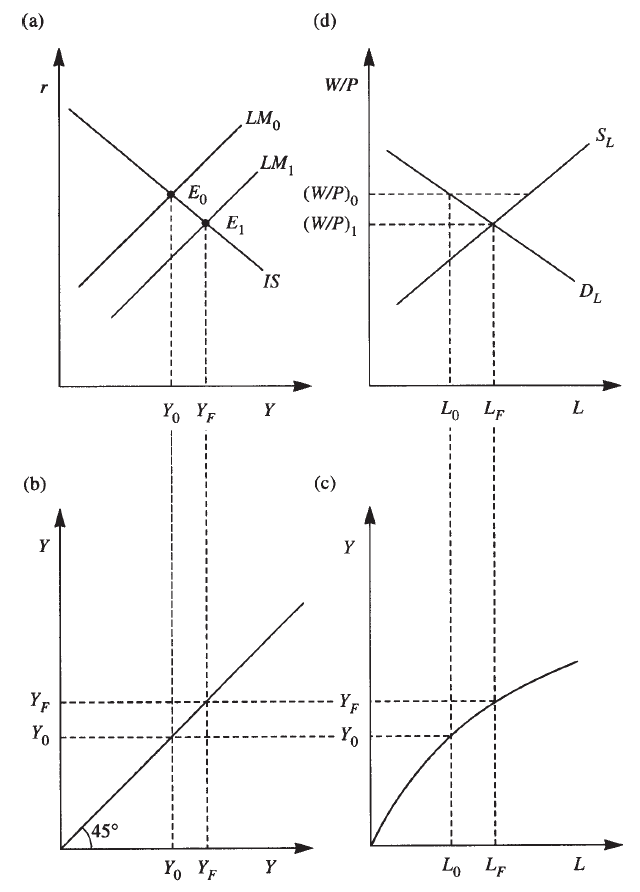
\includegraphics[width=0.3\textwidth]{./figures/aula7_fig1.PNG}
        \caption{Equilíbrio de subemprego no modelo IS-LM: caso geral e efeito Keynes. Fonte: Snowdon e Vane (2005).}
        \label{fig1}
    \end{figure}
\end{frame}

\begin{frame}{Equilíbrio de subemprego - IS-LM: caso geral}
    \begin{itemize}
        \item Leitura em sentido anti-horário a partir do quadrante (a) para determinar as implicações do nível de renda (determinado pela demanda agregada) em termos do nível de emprego no quadrante (d)
        \bigskip
        \item Economia em equilíbrio inicial: intersecção curvas IS e $LM_0$
        \bigskip
        \item Equilíbrio simultâneo nos mercados de bens e monetário evidencia que o nível de renda agregada de equilíbrio está abaixo do valor de pleno emprego $Y_F$
        \bigskip
        \item Quadrante (d) evidencia que sob um salário nominal fixo (exógeno) e um nível de preços consistente com o equilíbrio no mercado monetário (curva $LM_0$), o nível resultante de salário real $(W/P)_0$ é inconsistente com a condição de equilíbrio (\emph{market-clearing}) no mercado de trabalho
    \end{itemize}
\end{frame}

\begin{frame}{Equilíbrio de subemprego - IS-LM: caso geral}
    \begin{itemize}
        \item De outra forma, não há garantias de que o nível de emprego determinado pela demanda $L_0$ seja igual ao nível de pleno emprego $L_F$
        \bigskip
        \item O excesso de oferta de trabalho não tem efeito algum sobre o salário nominal, portanto, é possível que a economia permaneça em uma situação de equilíbrio abaixo do de pleno emprego, com desemprego persistente
        \bigskip
        \item Qual o efeito que a combinação do modelo IS-LM com a hipótese clássica de flexibilidade de preços e salários nominais tem sobre a possibilidade teórica de um equilíbrio de subemprego?
    \end{itemize}
\end{frame}

\begin{frame}{Equilíbrio de subemprego - IS-LM: caso geral}
    \begin{itemize}
        \item Partindo do equilíbrio inicial abaixo do pleno emprego, notamos um nível de emprego agregado $L_0$ abaixo do nível de pleno emprego $L_F$, com salários reais $(W/P)_0$ acima do valor de equilíbrio $(W/P)_1$
        \bigskip
        \item Desde que preços e salários sejam perfeitamente flexíveis, no entanto, o sistema econômico se auto-equilibrará no equilíbrio de pleno emprego
        \bigskip
        \item Ao nível de salário real $(W/P)_0$, o excesso de oferta de trabalho resultará em uma queda no salário nominal o que, por sua vez, reduz os custos das firmas e causa uma queda no nível de preços
        \bigskip
        \item A queda do nível de preços aumenta o valor real da oferta de moeda, deslocando a curva LM para a direita
    \end{itemize}
\end{frame}

\begin{frame}{Equilíbrio de subemprego - IS-LM: caso geral}
    \begin{itemize}
        \item O excesso de encaixes reais é canalizado para o mercado de títulos, onde os preços aumentam e a taxa de juros diminui
        \bigskip
        \item A queda na taxa de juros estimula gastos privados com investimento, aumentando o nível de demanda agregada e, consequentemente, o produto e o emprego
        \bigskip
        \item O efeito indireto da redução nos preços e salários nominais que estimula os gastos via taxa de juros é o que conhecemos como \hlight{efeito Keynes}
        \bigskip
        \item O aumento de DA modera a taxa de queda no nível de preços de modo que o salário nominal cai a uma taxa maior que a do nível de preços - deflação não-balanceada
    \end{itemize}
\end{frame}

\begin{frame}{Equilíbrio de subemprego - IS-LM: caso geral}
    \begin{itemize}
        \item O salário real, portanto, é reduzido na direção do nível de equilíbrio de pleno emprego $(W/P)_1$
        \bigskip
        \item Salários nominais e preços continuarão a declinar e a curva LM continuará a se deslocar para a direita até que o equilíbrio de pleno emprego é restaurado e o excesso de oferta de trabalho seja eliminado
        \bigskip
        \item É importante ressaltar que, \textcolor{blue}{é o aumento de DA, via efeito Keynes, que assegura que a economia retorne ao equilíbrio de pleno emprego}
    \end{itemize}
\end{frame}

\begin{frame}{Equilíbrio de subemprego - IS-LM: casos limites ou especiais}
    \begin{itemize}
        \item Nesta abordagem existem dois casos limites que, apesar da flexibilidade de preços e salários nominais, impedem o sistema econômico de se auto-equilibrar no nível de pleno emprego:
        \bigskip
        \begin{enumerate}
            \item Armadilha da liquidez.
            \bigskip
            \item Gastos com investimentos inelásticos com relação à taxa de juros.
        \end{enumerate}
    \end{itemize}
\end{frame}

\begin{frame}{Equilíbrio de subemprego - IS-LM: armadilha da liquidez}
    \begin{figure}
        \centering
        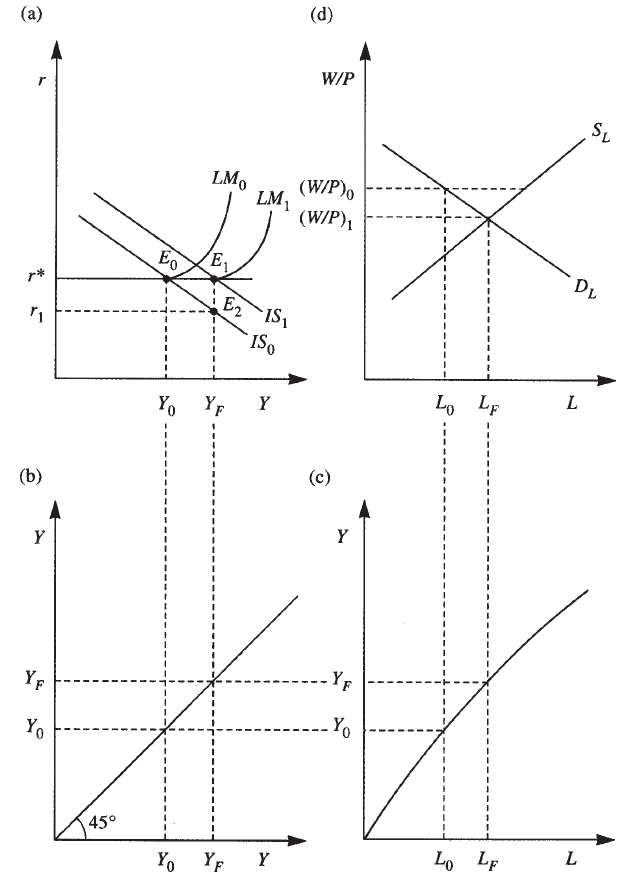
\includegraphics[width=0.3\textwidth]{./figures/aula7_fig2.PNG}
        \caption{Armadilha da liquidez. Fonte: Snowdon e Vane (2005).}
        \label{fig2}
    \end{figure}
\end{frame}

\begin{frame}{Equilíbrio de subemprego - IS-LM: armadilha da liquidez}
    \begin{itemize}
        \item Economia em equilíbrio inicial de subemprego
        \bigskip
        \item Ao salário real $(W/P)_0$ acima do equilíbrio, o excesso de oferta de trabalho resultará em queda de salários nominais que, por sua vez, reduz os custos das firmas e causa uma queda no nível de preços
        \bigskip
        \item Apesar de esta queda do nível de preços aumentar o valor real da oferta monetária (deslocando a curva LM para a direita), o aumento dos encaixes reais é inteiramente absorvido por encaixes ociosos ou especulativos
        \bigskip
        \item Em outras palavras, sob armadilha da liquidez, onde a demanda por moeda é perfeitamente elástica com relação à taxa de juros $r^*$, o excesso de encaixes reais não será canalizado para o mercado de títulos e isso irá impedir uma redução da taxa de juros para $r_1$ (que seria necessário para estimular a demanda agregada e restaurar o equilíbrio de pleno emprego)
    \end{itemize}
\end{frame}

\begin{frame}{Equilíbrio de subemprego - IS-LM: armadilha da liquidez}
    \begin{itemize}
        \item Como não há aumento de DA para moderar a taxa de declínio dos preços, o nível de preços é reduzido à mesma taxa que salários nominais - deflação balanceada
        \bigskip
        \item Salários reais mantidos em $(W/P)_0$ acima do valor de equilíbrio
        \bigskip
        \item \textcolor{blue}{DA insuficiente para alcançar pleno emprego - economia permanecerá em situação de subemprego com um desemprego involuntário persistente}
        \bigskip
        \item Sob armadilha da liquidez, a política monetária torna-se completamente ineficaz, enquanto a política fiscal alcança sua eficácia máxima como um meio de aumentar demanda agregada e, portanto, os níveis de produto e emprego agregados
    \end{itemize}
\end{frame}

\begin{frame}{Equilíbrio de subemprego - IS-LM: investimento inelástico}
    \begin{figure}
        \centering
        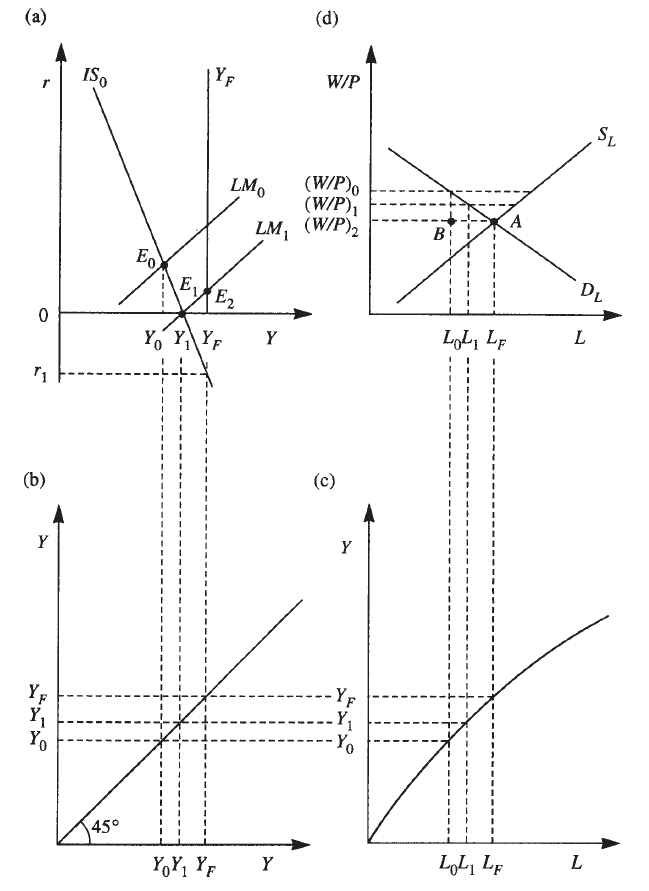
\includegraphics[width=0.3\textwidth]{./figures/aula7_fig3.PNG}
        \caption{Inelasticidade-juros do investimento. Fonte: Snowdon e Vane (2005).}
        \label{fig3}
    \end{figure}
\end{frame}

\begin{frame}{Equilíbrio de subemprego - IS-LM: investimento inelástico}
    \begin{itemize}
        \item Investimento inelástico com relação à taxa de juros: sistema econômico também será impedido de se auto-equilibrar no nível de pleno emprego
        \bigskip
        \item Economia em equilíbrio inicial de subemprego
        \bigskip
        \item Ao salário real $(W/P)_0$ acima do equilíbrio, o excesso de oferta de trabalho resultará em uma queda de salários nominais que, por sua vez, reduz os custos das firmas e causa uma queda no nível de preços
        \bigskip
        \item Apesar do aumento no valor real da oferta monetária (que desloca LM para a direita) via efeito Keynes resultar em uma redução da taxa de juros, esta queda na taxa de juros é insuficiente para restaurar o equilíbrio de pleno emprego
    \end{itemize}
\end{frame}

\begin{frame}{Equilíbrio de subemprego - IS-LM: investimento inelástico}
    \begin{itemize}
        \item Figura \ref{fig3} revela que, com investimento tão inelástico com relação aos juros, o equilíbrio de pleno emprego só poderia ser restaurado via efeito Keynes com uma taxa de juros negativa em $r_1$
        \bigskip
        \item Na teoria, \textcolor{blue}{o sistema econômico convergiria para um equilíbrio estável no ponto $E_1$ - com uma taxa de juros igual a zero - um ponto de equilíbrio de subemprego com desemprego involuntário persistente}
    \end{itemize}
\end{frame}

\begin{frame}{Equilíbrio de subemprego - IS-LM: resumo}
    \begin{itemize}        
        \item Em resumo, \textcolor{blue}{reduções nos salários nominais e no nível de preços serão insuficientes para restaurar o equilíbrio de pleno emprego a não ser que consigam aumentar a DA via efeito Keynes}
        \bigskip
        \item \textcolor{blue}{Nos casos de armadilha da liquidez e inelasticidade-juro do investimento, a DA é insuficiente para alcançar o pleno emprego e, portanto, o desemprego involuntário só será eliminado se o nível de DA é aumentado via uma política fiscal expansionista}
    \end{itemize}
\end{frame}

\begin{frame}{Equilíbrio de subemprego - IS-LM: resumo}
    \begin{itemize}
        \item O efeito de combinar o modelo de estática-comparativa IS-LM com a hipótese clássica de flexibilidade perfeita de preços e salários nominais é evidenciar que \textcolor{blue}{Keynes não obteve sucesso em fornecer uma `teoria geral' de equilíbrio de subemprego robusta e que a possibilidade de um equilíbrio de subemprego depende de dois casos limites/especiais}
        \bigskip
        \item A análise anterior de equilíbrio, derivada em grande parte da obra de Modigliani, implica que é possível para o sistema econômico convergir para um equilíbrio estável com desemprego involuntário persistente no caso em que impomos algum tipo de rigidez ao sistema
        \bigskip
        \item Isto é, se assumirmos rigidez nominal de salários, armadilha da liquidez ou investimento inelástico com relação aos juros
    \end{itemize}
\end{frame}

\begin{frame}{Equilíbrio de subemprego - IS-LM: resumo}
    \begin{itemize}
        \item Em contraste, Patinkin (1956) argumentou que o desemprego é um fenômeno de desequilíbrio e pode prevalecer mesmo quando preços e salários nominais são perfeitamente flexíveis
        \bigskip
        \item Para ilustrar o argumento, assuma uma posição inicial de pleno emprego
        \bigskip
        \item Suponha, então, que haja uma redução de DA
        \bigskip
        \item Essa redução de DA resultará em um período de desequilíbrio no qual tantos os preços quanto os salários nominais tenderão a sofrer uma redução
        \bigskip
        \item Patinkin assume que salários nominais e nível de preços irão ser reduzidos à mesma taxa - deflação balanceada
        \bigskip
        \item Consequentemente, a queda no nível agregado de emprego não está associada a um aumento de salário real, mas com a queda no nível agregado de demanda efetiva
    \end{itemize}
\end{frame}

\begin{frame}{Equilíbrio de subemprego - IS-LM: resumo}
    \begin{itemize}
        \item De outra forma, firmas serão forçadas para fora de suas curvas de demanda por trabalho
        \bigskip
        \item Considerando o quadrante (d) da Figura \ref{fig3}, isso levaria a um movimento do ponto $A$ para o ponto $B$
        \bigskip
        \item No entanto, na visão de Patinkin, essa condição de desequilíbrio não será mantida indefinidamente
        \bigskip
        \item Pois a queda de preços e salários nominais leva a um `efeito direto' estimulando um aumento de DA, via valor dos encaixes monetários e, com isso, restaurando o pleno emprego (movimento do ponto $B$ de volta para o ponto $A$)
        \bigskip
        \item Essa versão particular do efeito riqueza sobre os gastos é conhecida como \textcolor{blue}{efeito de encaixes reais}
    \end{itemize}
\end{frame}

\begin{frame}{Equilíbrio de subemprego - IS-LM: resumo}
    \begin{itemize}
        \item De maneira mais geral, a introdução de um \textcolor{blue}{efeito riqueza} ou \textcolor{blue}{efeito Pigou} sobre os gastos assegura que desde que preços e salários reais sejam flexíveis, mesmo nos casos limites, a economia irá se auto-equilibrar no ponto de pleno emprego
        \bigskip
        \item Discutiremos, então, a natureza e papel do efeito Pigou com relação à possibilidade de equilíbrio de subemprego no modelo IS-LM Keynesiano
    \end{itemize}
\end{frame}

\subsection{Efeito Pigou}
\begin{frame}{Efeito Pigou}
    \begin{columns}
% Column 1
\begin{column}{0.5\textwidth}
        \begin{itemize}
            \item Pigou foi um dos últimos principais economistas clássicos
            \bigskip
            \item Durante os anos 1940s, em suas contribuições para a escola clássica, argumentava que caso preços e salários nominais fossem flexíveis, o modelo Keynesiano ortodoxo não poderia se estabilizar em um equilíbrio abaixo do de pleno emprego
        \end{itemize}
\end{column}
% Column 2    
\begin{column}{0.5\textwidth}
    \begin{figure}
    \centering
        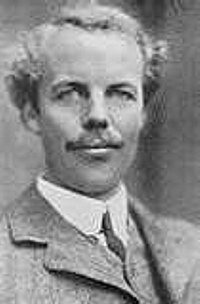
\includegraphics[width=0.5\textwidth]{./figures/aula7_fig4.jpg}
        \caption{Arthur Cecil Pigou (1877-1959).}
        \label{fig4}
    \end{figure}
\end{column}
\end{columns}
\end{frame}

\begin{frame}{Efeito Pigou}
    \begin{itemize}
        \item O \textcolor{blue}{efeito Pigou} está relacionado ao efeito positivo que uma queda de preços tem sobre a riqueza real o que, por sua vez, aumenta os gastos de consumo
        \bigskip
        \item Suponha economia em equilíbrio inicial de pleno emprego e sob armadilha da liquidez - Figura \ref{fig2}
        \bigskip
        \item O excesso de oferta de trabalho reduz o salário nominal e os custos das firmas, reduzindo o nível de preços
        \bigskip
        \item A queda do nível de preços não só desloca a curva LM para a direita à medida que o valor real da oferta de moeda aumenta
        \bigskip
        \item A curva IS também é deslocada para a direita, já que o aumento da riqueza total resultante aumenta os gastos com consumo
    \end{itemize}
\end{frame}

\begin{frame}{Efeito Pigou}
    \begin{itemize}
        \item Na teoria, a economia não pode se estabilizar em um equilíbrio de subemprego
        \bigskip
        \item Teremos, então, um ajuste automático até que o equilíbrio de pleno emprego seja atingido, no ponto de intersecção entre as curvas $IS_1$ e $LM_1$ - ponto $E_1$
        \bigskip
        \item De maneira similar, ao incorporarmos o efeito Pigou (ou efeito riqueza) sobre o consumo à nossa análise, o caso especial de investimento inelástico com relação à taxa de juros ilustrado pela Figura \ref{fig3} também irá se ajustar automaticamente para restaurar o pleno emprego no ponto $E_2$
    \end{itemize}
\end{frame}

\begin{frame}{Efeito Pigou}
    \begin{itemize}
        \item A importância teórica do efeito Pigou pode ser, então, assim sumarizado:        \bigskip
        \begin{flushright}
            \NB{
            O efeito Pigou finalmente descarta a controv\'{e}rsia Keynesiana de que o equil\'{i}brio de pleno emprego n\~{a}o depende da hip\'{o}tese de rigidez nominal de sal\'{a}rios. Depende.
        \begin{flushright}
            (Johnson, 1964).
        \end{flushright}}
        \end{flushright}
    \end{itemize}
\end{frame}

\begin{frame}{Efeito Pigou: limitações}
    \begin{itemize}
        \item Destacaremos duas das principais limitações identificadas à capacidade do efeito Pigou em assegurar um retorno ao equilíbrio de pleno emprego
        \bigskip
        \item[1.] Considerações dinâmicas podem invalidar o efeito Pigou como um mecanismo auto-equilibrador:
        \bigskip
        \begin{enumerate}
            \item[1.1.] Se indivíduos antecipam uma queda futura do nível de preços, eles podem postergar consumo corrente e, com isso, levando a um aumento do desemprego
            \bigskip
            \item[1.2.] Ao mesmo tempo, se firmas esperam que o período de recessão se prolongue, elas podem postergar seus planos de investimento o que, também, eleva a taxa de desemprego
            \bigskip
            \item[1.3.] Além disso, em períodos de recessão profunda, o número de falências tende a aumentar, reduzindo a despesa agregada ainda mais
        \end{enumerate}
    \end{itemize}
\end{frame}

\begin{frame}{Efeito Pigou: limitações}
    \begin{itemize}
        \item I.e., a queda do nível de preços pode levar a um deslocamento da curva IS para a esquerda, distanciando a economia ainda mais do equilíbrio de pleno emprego
        \bigskip
        \item Nestas circunstâncias, políticas fiscais expansionistas assegurariam um retorno ao equilíbrio de pleno emprego mais rápido
        \bigskip
        \item[2.] Breve consideração do debate sobre quais tipos de ativos constituem \textcolor{blue}{riqueza líquida}
        \bigskip
        \item A \textcolor{blue}{riqueza líquida} pode ser definida como a riqueza total subtraída dos passivos pendentes
    \end{itemize}
\end{frame}

\begin{frame}{Efeito Pigou: limitações}
    \begin{itemize}
        \item No modelo Keynesiano, a riqueza pode ser mantida sob a forma de moeda e sob a forma de títulos
        \bigskip
        \item Consideraremos, inicialmente, a moeda que pode ser definida como papel-moeda em poder do público somado a depósitos bancários
        \bigskip
        \item \textcolor{blue}{Moeda externa} (\emph{outside money}): moeda que é um passivo direto sobre o setor público (e.g., papel-moeda em poder do público) e/ou moeda baseada em dívidas do setor público (e.g., depósitos bancários que são equalizados pelas reservas dos bancos ou reservas juntas ao BC)
        \bigskip
        \item \textbf{Portanto, a moeda externa pode ser considerada como riqueza líquida do setor privado dado que não existe uma contrapartida de passivos do setor privado}.
    \end{itemize}
\end{frame}

\begin{frame}{Efeito Pigou: limitações}
    \begin{itemize}
        \item \textcolor{blue}{Moeda interna} (\emph{inside money}): moeda que é baseada em dívidas do setor privado. O principal exemplo de moeda interna são os depósitos de bancos comerciais que são equalizados por passivos do setor privado de igual magnitude - empréstimos bancários para tomadores de empréstimos do setor privado
        \bigskip
        \item Como estes depósitos bancários são compensados por passivos do setor bancário (empréstimos bancários), podemos argumentar que a moeda interna não constitui riqueza líquida
        \bigskip
        \item Cabe ressaltar, no entanto, que o argumento de que moeda interna não constitui riqueza líquida tem sido questionado por alguns economistas como Pesek e Saving (1967) e Johnson (1969)
    \end{itemize}
\end{frame}

\begin{frame}{Efeito Pigou: limitações}
    \begin{itemize}
        \item Se assumirmos que riqueza líquida só é constituída por moeda externa, fica evidente que o efeito riqueza resultante de uma trajetória de queda dos preços é reduzido consideravelmente
        \bigskip
        \item Feita a discussão acerca dos agregados monetários que podem ser considerados riqueza líquida consideraremos, agora, o debate sobre se títulos públicos podem ser tratados como riqueza líquida
        \bigskip
        \item Como vimos anteriormente, podemos argumentar que o setor privado irá perceber que, seguindo uma queda de preços, o aumento do valor real da dívida pública em circulação irá requerer aumentos futuros dos impostos para arcar com o aumento do valor de pagamentos de juros da dívida e, também, os resgates destes títulos públicos
    \end{itemize}
\end{frame}

\begin{frame}{Efeito Pigou: limitações}
    \begin{itemize}
        \item Se o valor presente dos gastos futuros com tributos compensar, exatamente, o aumento do valor real da dívida em circulação, então, não existirá nenhum deslocamento da curva IS induzido por efeito riqueza
        \bigskip
        \item Apesar de esta visão não ser amplamente aceita, ela coloca dúvidas sobre as propriedades auto-equilibradoras da economia via efeito Pigou
        \bigskip
        \item De fato, a evidência empírica sugere que o efeito Pigou é extremamente fraco
        \bigskip
        \item Os resultados obtidos por Glahe (1973) para os EUA e Morgan (1978) para o UK mostraram que o efeito Pigou não era forte o suficiente para restaurar o equilíbrio de pleno emprego no período do entre-guerras - quedas do nível de preços correntes ocorrem conjuntamente com declínios dos gastos e renda agregada
    \end{itemize}
\end{frame}

\begin{frame}{Efeito Pigou: limitações}
    \begin{itemize}
        \item Stiglitz (1992) mostrou que, se o nível de preços sofre uma redução de 10\% ao ano, então, \emph{ceteris paribus}, ``para aumentar o nível de consumo em 25\% levaria, aproximadamente, 400 anos''
        \bigskip
        \item Portanto, ``é difícil perceber, mesmo sob a visão mais otimista, a significância quantitativa do efeito de encaixes reais para a análise macroeconômica de curto prazo''
        \bigskip
        \item Dadas estas dúvidas e limitações, \textcolor{blue}{a prescrição de política macroeconômica dos economistas Keynesianos é de uma política fiscal expansionista para assegurar uma convergência mais rápida ao equilíbrio de pleno emprego}
    \end{itemize}
\end{frame}

\subsection{A síntese neoclássica}
\begin{frame}{A síntese neoclássica}
    \begin{itemize}
        \item De toda a discussão que fizemos até agora, percebemos que se o salário nominal e os preços são perfeitamente flexíveis, o modelo IS-LM Keynesiano pode, em teoria, via efeito riqueza ou efeito Pigou, automaticamente se ajustar para alcançar o equilíbrio de pleno emprego - a principal predição da macroeconomia clássica
        \bigskip
        \item Pigou parece ter vencido o debate teórico
        \bigskip
        \item No entanto, Keynesianos parecem ter vencido o debate político dado que o ajuste via efeito Pigou poderia ser tão lento que políticas intervencionistas (mais notavelmente, políticas fiscais expansionistas) seriam necessárias para assegurar um retorno mais rápido ao pleno emprego
    \end{itemize}
\end{frame}

\begin{frame}{A síntese neoclássica}
    \begin{itemize}
        \item No final dos anos 1950s e início dos 1960s, uma visão consensual emergiu - \textcolor{blue}{síntese neoclássica}
        \bigskip
        \item Segundo esta visão, a Teoria Geral seria vista como um caso específico de uma teoria clássica mais geral (ou seja, o caso em que a rigidez de reduções de salários nominais impede o processo de ajuste automático clássico ao pleno emprego)
        \bigskip
        \item Enquanto a necessidade de políticas intervencionistas Keynesianas foi reconhecida para assegurar uma convergência mais rápida ao pleno emprego
    \end{itemize}
\end{frame}

\section{Bibliografia}
\begin{frame}{\emoji{books} Bibliografia}
    \begin{itemize}                
        %\item DE VROEY, M. \emph{A History of Macroeconomics from Keynes to Lucas and Beyond}. Cambridge University Press, 2016.\medskip        
        \item GLAHE, F.R. Macroeconomics: Theory and Policy, New York: Harcourt Brace Jovanovich, 1973.\medskip
        \item JOHNSON, H.G. Money, Trade and Economic Growth, London: Allen and Unwin, 1964.\medskip
        \item JOHNSON, H.G. Inside Money, Outside Money, Income, Wealth and Welfare in Monetary Theory, Journal of Money, Credit, and Banking, February, 1969\medskip
        \item MORGAN, B. Monetarists and Keynesians: Their Contribution to Monetary Theory, London: Macmillan, 1978.\medskip
        \item PATINKIN, D. Money, Interest and Prices: An Integration of Monetary and Value Theory, Evanston, IL: Row Peterson, 1956.\medskip
        \item PESEK, B.; SAVING, T.R. Money, Wealth and Economic Theory, London: Macmillan, 1967\medskip
        \item SNOWDON, B.; VANE, H.R. An encyclopedia of macroeconomics. Northampton, USA: Edward Elgar Publishing Limited, 2002.\medskip
        \item SNOWDON, B.; VANE, H.R. \emph{Modern Macroeconomics: its Origins, Development and Current State}. Northampton, MA: Edward Elgar, 2005.\medskip
        \item STIGLITZ, J.E. Methodological Issues and the New Keynesian Economics, in A. Vercelli and N. Dimitri (eds), Macroeconomics: A Survey of Research Strategies, Oxford: Oxford University Press, 1992.
    \end{itemize}
\end{frame}
\end{document}